\chapter{Facility Description}
\label{vl:tc-facility}


\section{Detector Caverns Cryostats and Cryogenics}
\label{sec:fdsp-coord-faci-caverns}


The underground facilities for the detectors consist of two parallel
detector caverns and one central utility cavern between them. The long
direction of the caverns is aligned approximately in the east-west
direction. Therefore, the two detector caverns are named north and
south caverns. Figure~\ref{fig:dune-underground} shows the overall
underground campus.
\begin{dunefigure}[Underground campus]{fig:dune-underground}
  {Underground campus at the 4850 level.}
  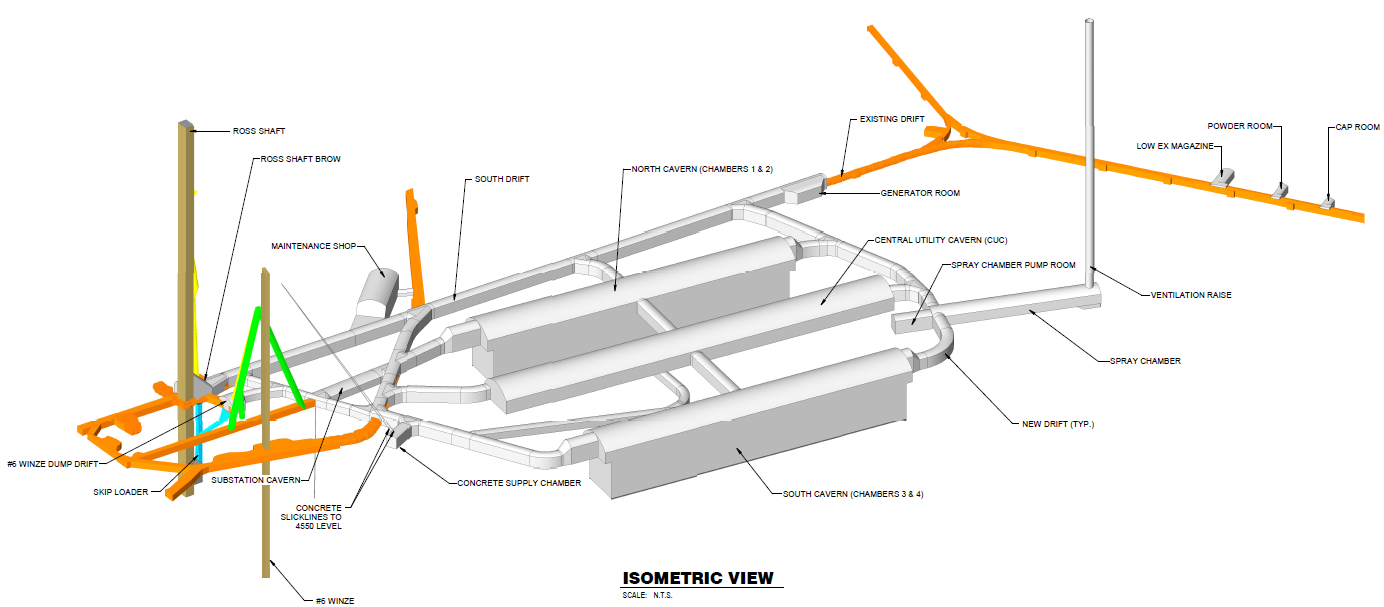
\includegraphics[width=0.85\textwidth]{Underground_campus.png}
\end{dunefigure}


Each detector cavern is \SI{144.5}{\meter} long, \SI{19.8}{\meter}
wide and \SI{27.95}{\meter} high and will house two detector modules,
one on the west side and one on the east side. In between the two
detector modules in one cavern, there is a \SI{12}{\meter} space which
will be used for access to detectors, for cryogenic distribution pumps
and for atemporary clean room for detector installation. There are
access tunnels at the east and west ends of each cavern, north and
south side of north cavern and north side of south cavern.


The central utility cavern (CUC) is \SI{190}{\meter} long, \SI{19.3}{\meter}
wide, \SI{10.95}{\meter} high and will house cryogenic equipment, DAQ
room, and mechanical and electrical services for all four
detectors.


Each detector is housed inside a cryostat. Each cryostat is made from
outside to inside of: an external steel structure, a warm membrane
plate, insulation and a cold membrane. Figure~\ref{fig:dune-cryostat}
shows the overall construction. The cryostat will have a vertical
opening at one end which will allow installation of detector
components. The opening will be closed after completion of
installation and prior to filling.
\begin{dunefigure}[\dword{dune} cryostat]{fig:dune-cryostat}
  {Overall construction and dimensions of the \dword{dune} cryostat.}
  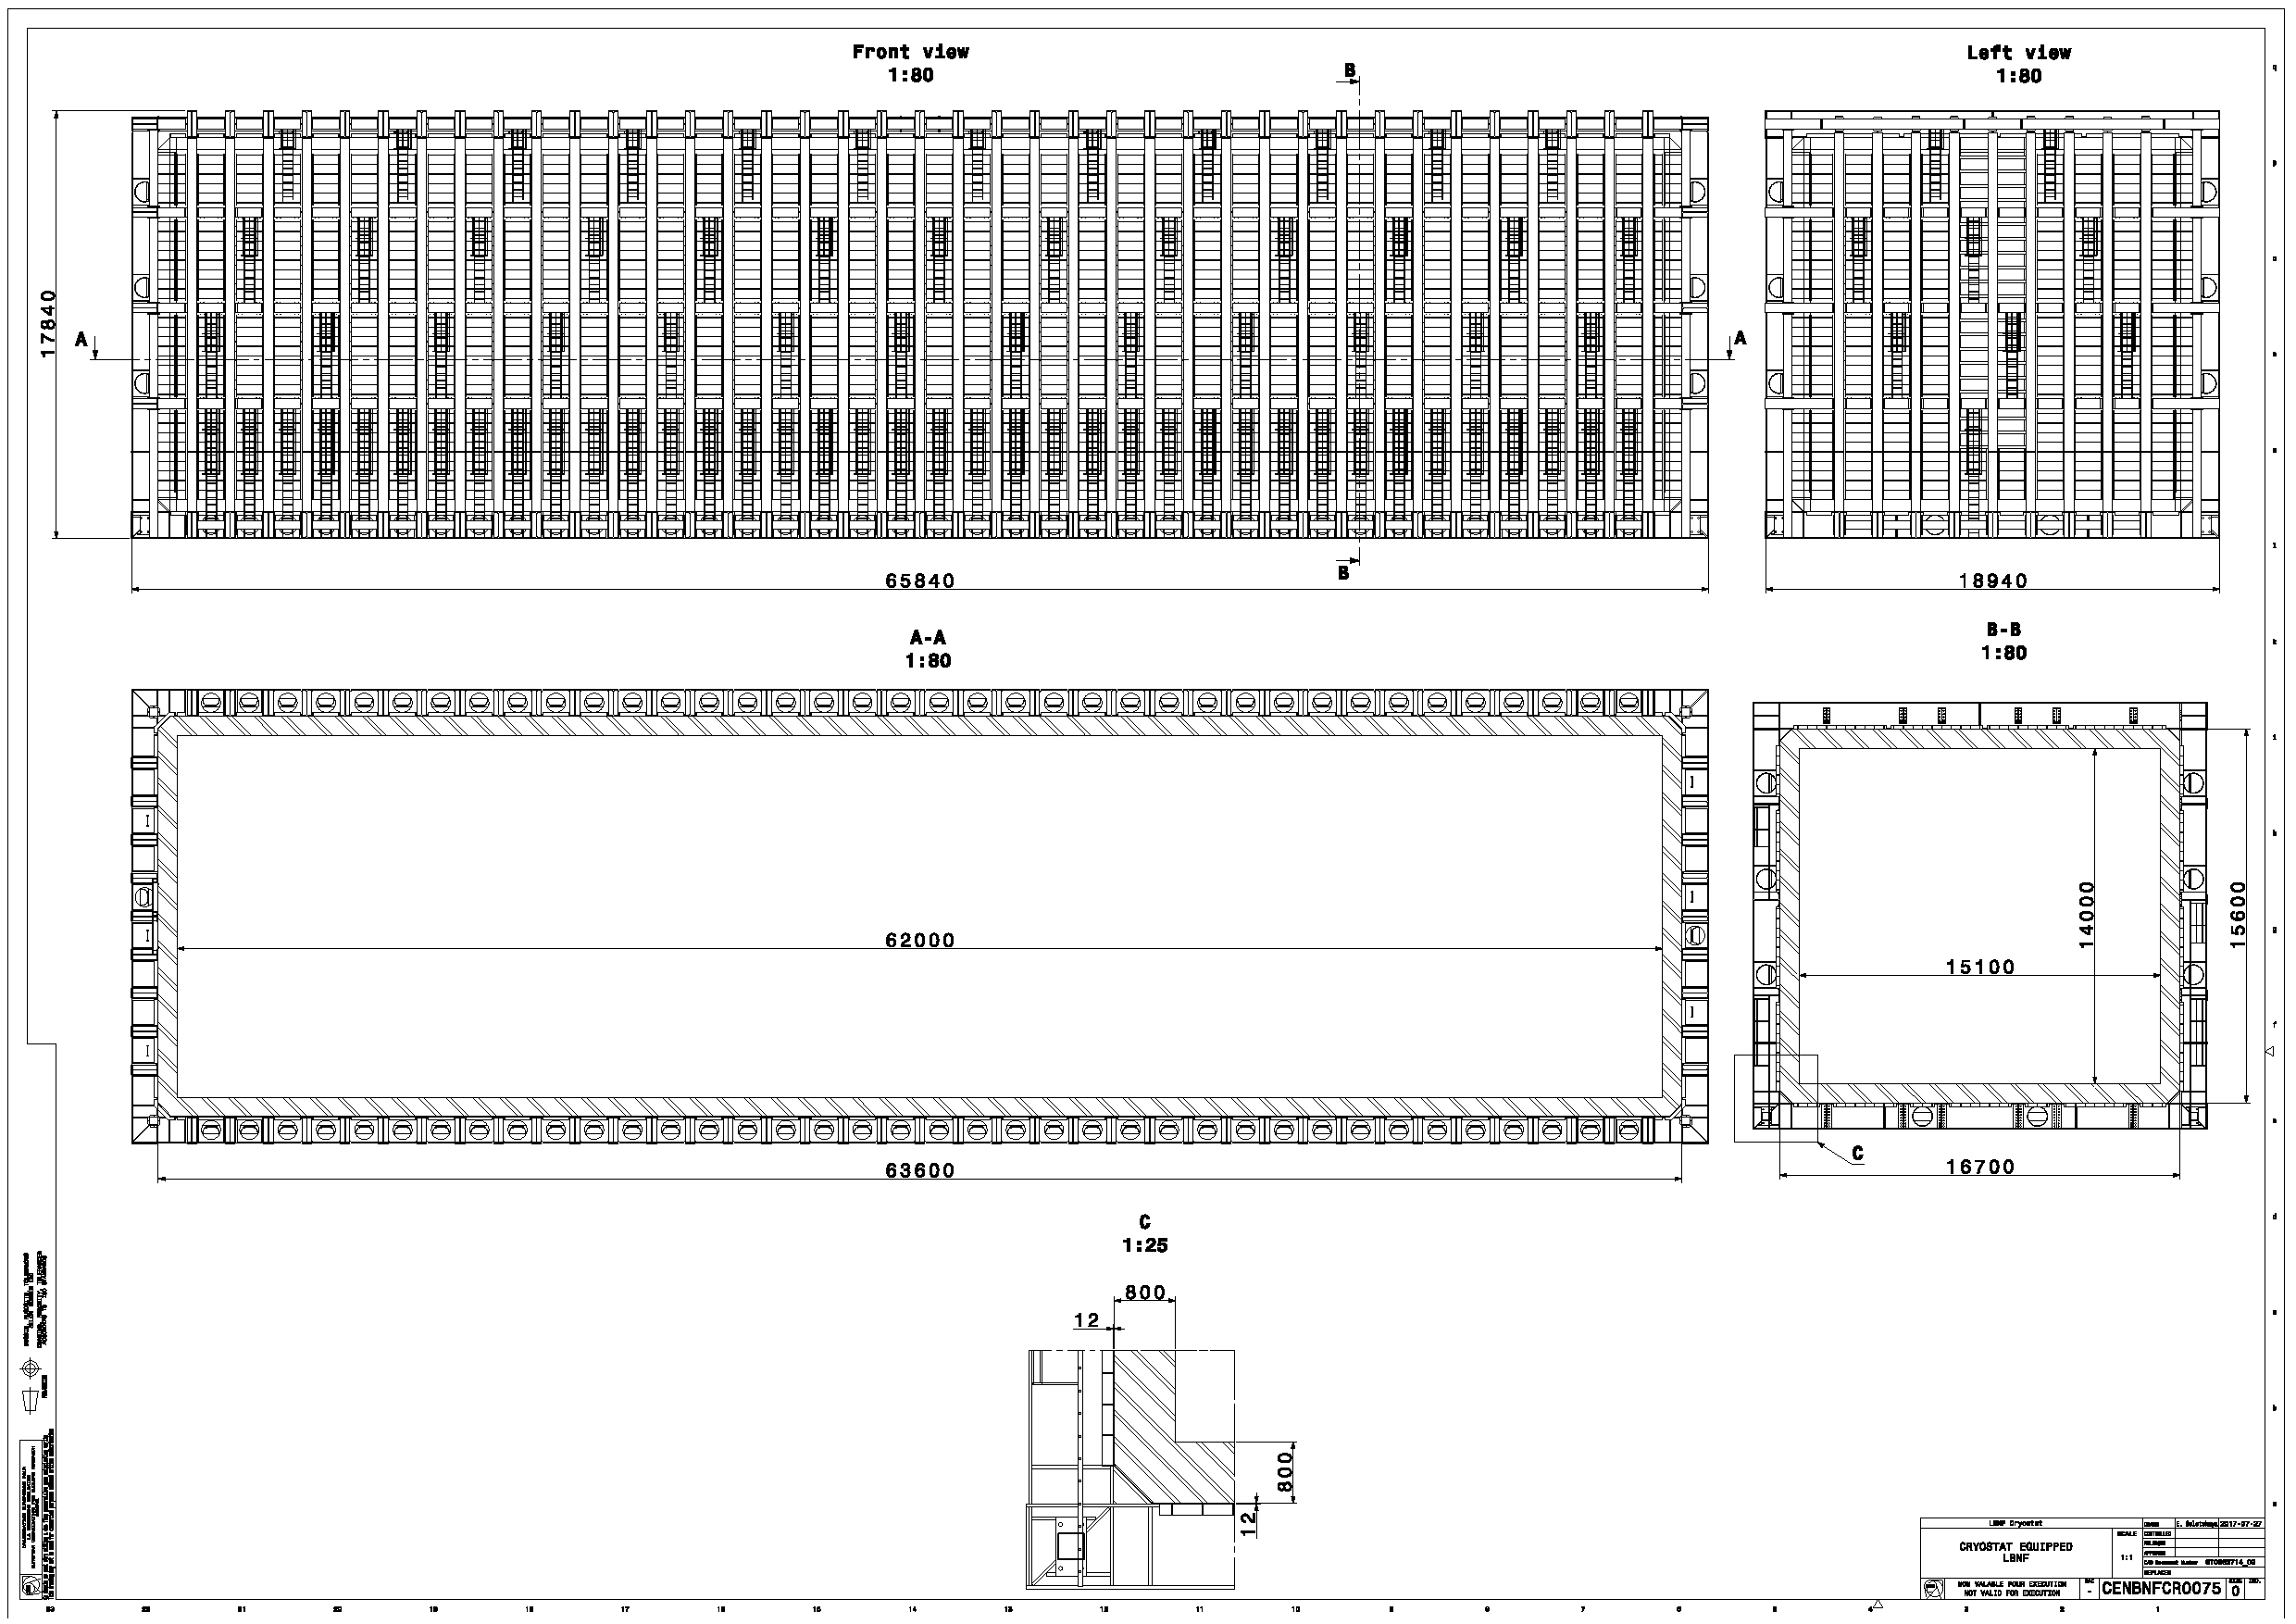
\includegraphics[width=0.85\textwidth]{cryostat.pdf}
\end{dunefigure}


The detector cryogenics system supplies liquid Argon and provides
circulation, re-condensation and purification. The cryogenic system
components are housed inside the CUC, on top of each detector module
and between detector modules. The cryogenic system is composed of:
\begin{itemize}
\item Infrastructure cryogenics, which includes LAr and LN$_2$ receiving
  facilities on the surface, nitrogen refrigeration system (split
  between above ground and underground), LN$_2$ buffer storage
  underground, LN$_2$, GN$_2$ and GAr piping to interconnect equipment and
  components in the detector cavern and the CUC, and process controls,
  integration and supporting equipment.
\item Proximity cryogenics, which includes reliquefaction and
  purification subsystems for the argon (gas and liquid), associated
  instrumentation and monitoring equipment, and LAr piping to
  interconnect equipment and components in the detector cavern and the
  CUC. The proximity cryogenics is split into multiple areas: in the
  CUC, on top of the mezzanine, on the side of the cryostat which is
  where LAr circulation pumps are located.
\item Internal cryogenics, which includes LAr and GAr distribution
  systems inside the cryostat, as well as features to cool down the
  cryostat and the detector uniformly.
\end{itemize}
Figure~\ref{fig:dune-cryogenics} shows the process flow diagram of the
\dword{lbnf} cryogenic system. Only one cryostat is shown for simplicity.
Figure~\ref{fig:dune-cryogenics}.
\begin{dunefigure}[Cryogenics system]{fig:dune-cryogenics}
  {Overall process flow diagram of the cryogenic system showing one
    cryostat only, other cryostats are the same.}
  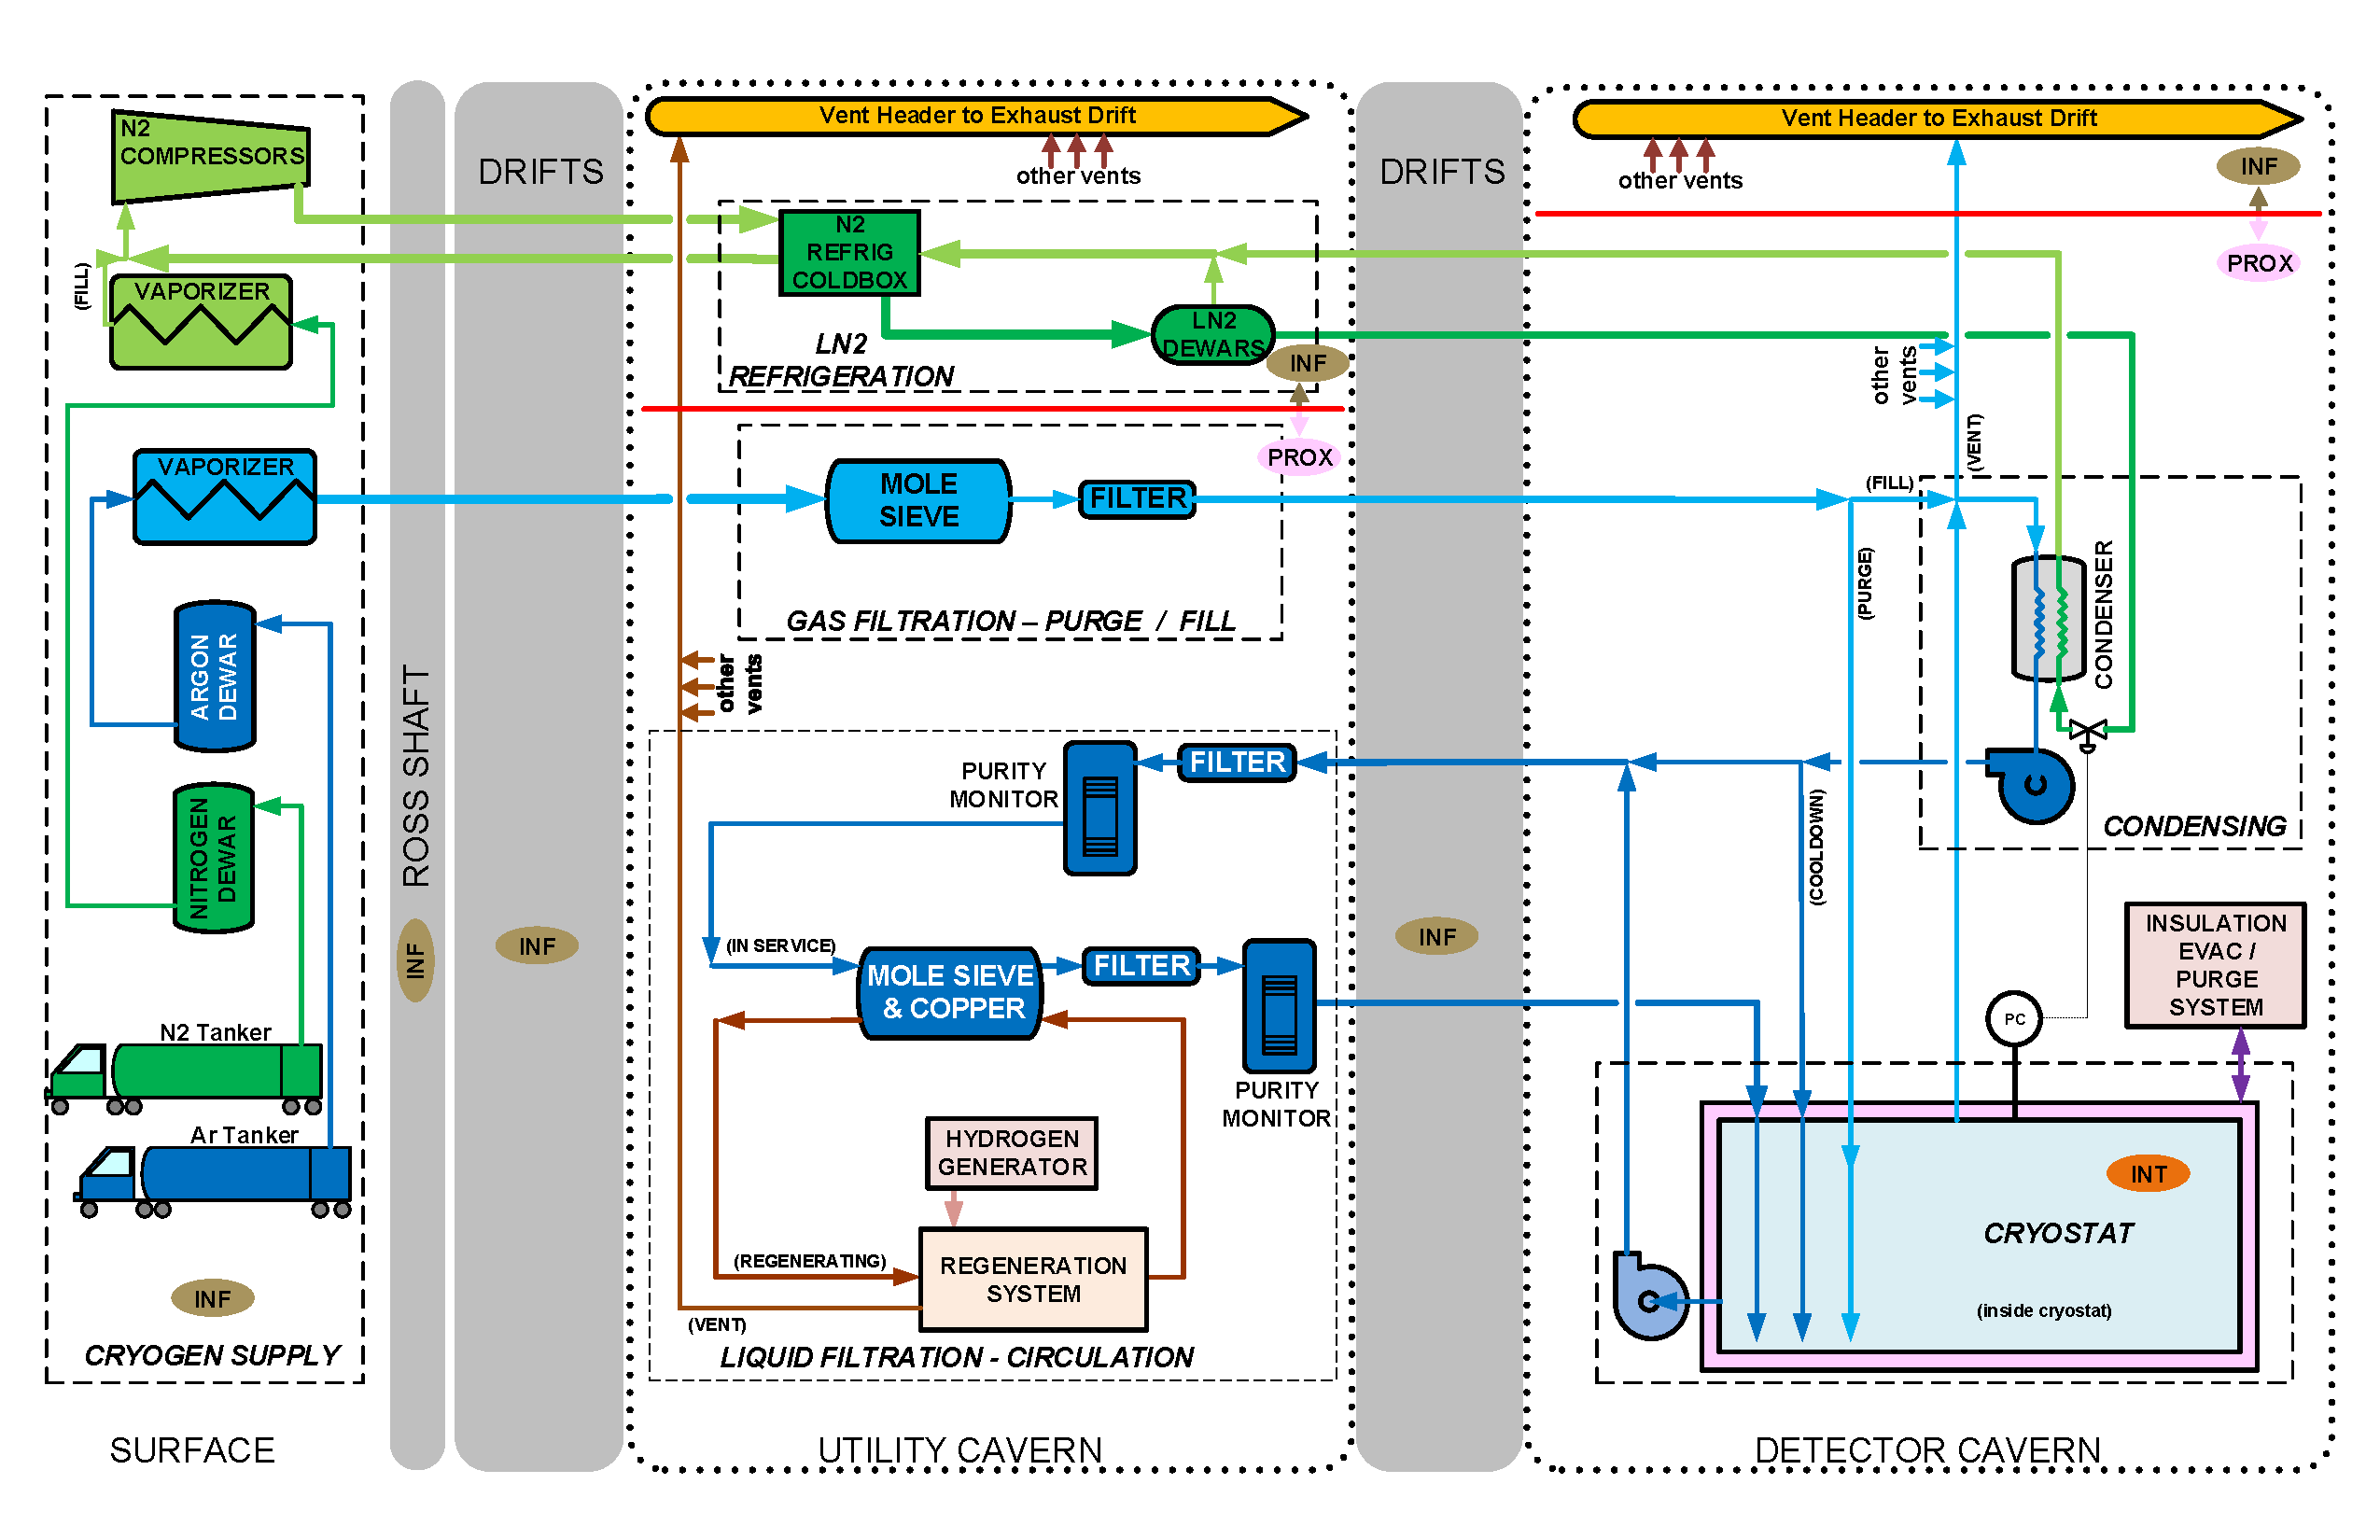
\includegraphics[width=0.85\textwidth]{LBNF_PFD_180909.pdf}
\end{dunefigure}


The underground facilities also include all the Building and Site
Infrastructure (BSI) and utilities, such as HVAC systems for
underground environment control, chilled water for cooling of detector
electronics and cryogenics compressors, material handling equipment
(monorails and bridge cranes), industrial water systems, lighting,
etc., required for detector construction and operation.


\section{Detector Grounding}
\label{sec:fdsp-coord-faci-grounding}


A detector grounding strategy has been adopted which will provide the
detector with an independent ``isolated'' ground to minimize any
environmental electrical noise which can couple into the detector
electronics either conductively or through emitted electromagnetic
interference.


The detectors will be located at the 4850 level of the Sanford
Underground Research Facility. The electrical conductivity of the
various rock masses are unknown but expected to have extremely poor
and inconsistent conductive properties. To insure adequate sensitivity
of the detectors, a special ground system must be put in place that
will isolate the detectors from all other electrical systems and
equipment, minimize the influence of inductive and capacitive coupling
and eliminate ground loops. The objective of the grounding
infrastructure requirements is to reduce or eliminate ground currents
through the detector which will affect detector sensitivity, maintain
a low impedance current path for equipment short circuit and ground
fault currents, and insure personnel safety by limiting
equipment-to-equipment and equipment-to-ground touch potentials.


Three basic ground structures have been identified which effect the
construction of the caverns.  These are shown in
Figure~\ref{fig:dune-grounding}.
\begin{dunefigure}[Overall \dword{dune} grounding structure]{fig:dune-grounding}
  {Overall \dword{dune} grounding structure incorporated in cavern.}
  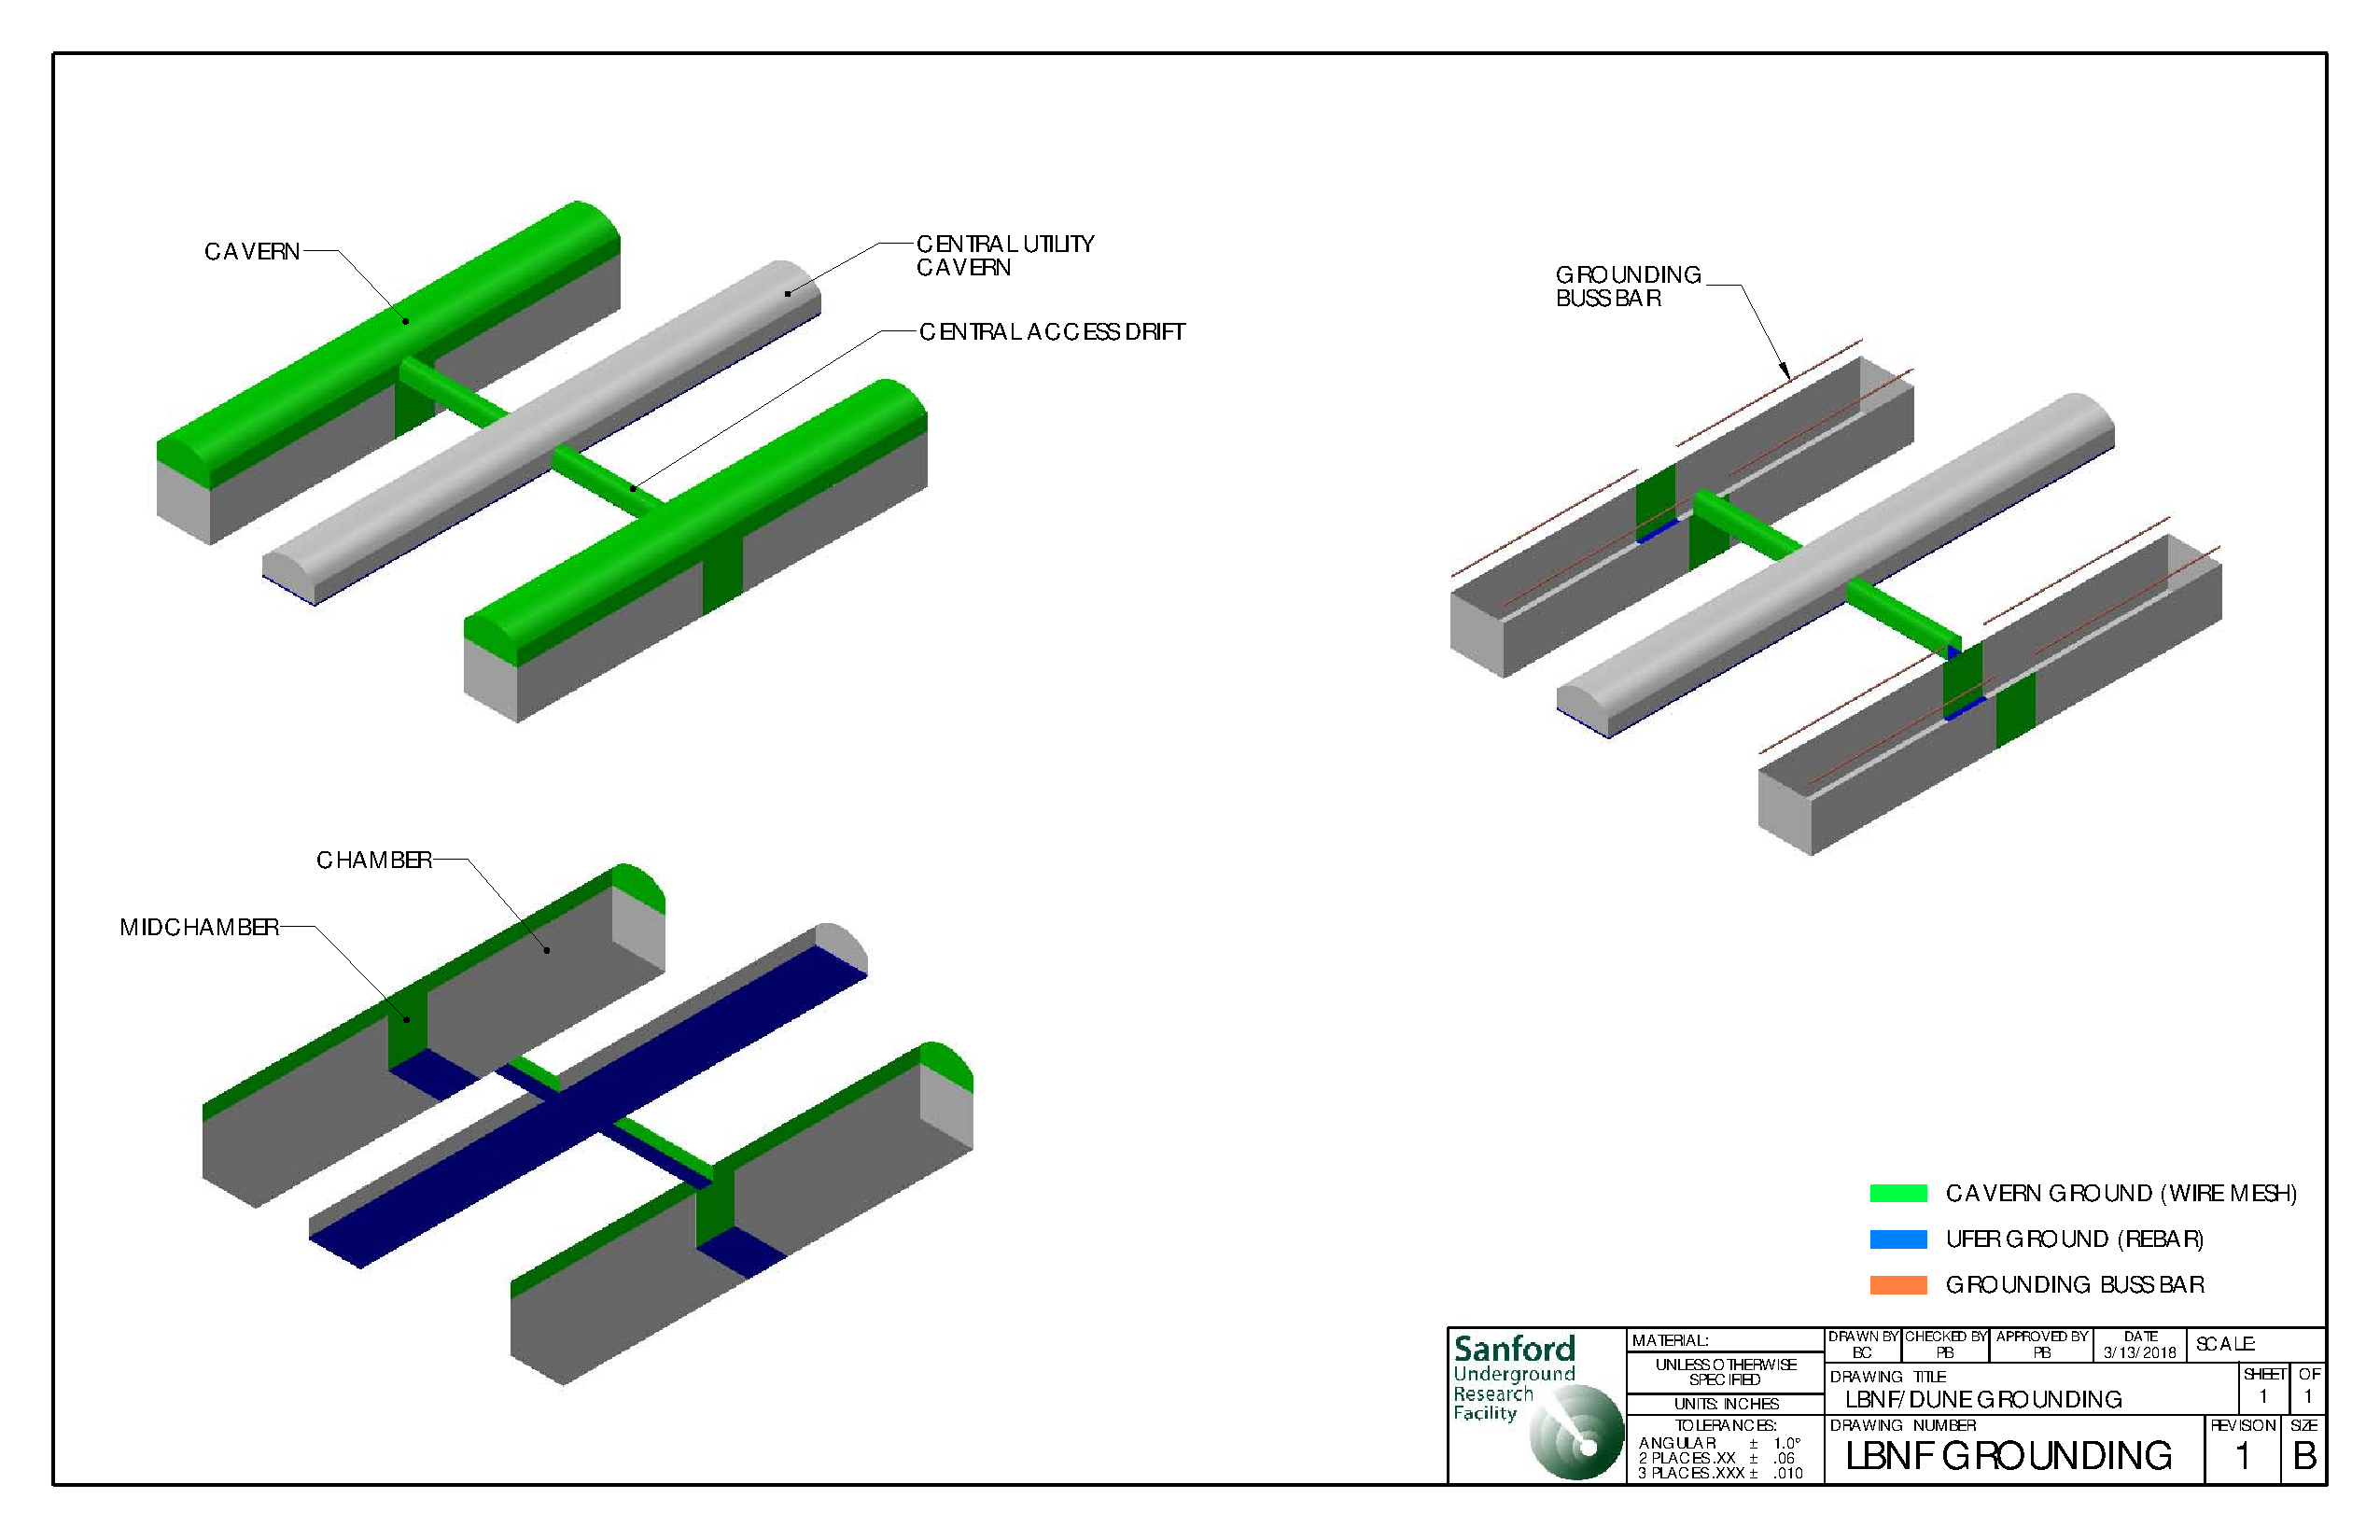
\includegraphics[width=0.85\textwidth]{SURF_Grounding.pdf}
\end{dunefigure}


These include:
\begin{enumerate}
 \item Cavern ground which consists of overlapping welded wire mesh
   supported by rock bolts and covered with shotcrete. The
   \dword{lbnf}/\dword{dune} Cavern ground includes all walls and
   crown areas above the 4850 level in the North and South detector
   caverns and their associated central access drifts, plus tin-plated
   copper bus bars specified to run the length of the detector vessels
   on each side along the cavern walls and mounted external to the
   shotcrete.  The Cavern ground structure:
\begin{enumerate}
 \item Spans the full length of the cavern from the West end access
   drift entrance through the mid-chamber to the East end access drift
   entrance.
 \item Spans the full width of the cavern from the 4850 level sill
   (top of the detector vessels and mid-chamber floor) on both sides
   up and across the crown of the cavern.
 \item Includes mid chamber walls to the 4910 level.
 \item Includes the east and west end walls of the cavern, from the
   4850 level to the crown.
\end{enumerate}
 \item Ufer ground which consists of the metal rebar embedded in the
   concrete floors. The \dword{lbnf}/\dword{dune} Ufer ground system
   includes the concrete floors in the cavern mid-chambers, center
   access drifts, and central utility cavern. The cavern and Ufer
   grounds will be electrically well bonded to construct a single
   facilities ground which will be isolated from detector ground.
 \item Detector ground consists of the steel containment vessel
   enclosing the cryostat and all metal structures attached to or
   supported by the detector vessel.
\end{enumerate}


To maintain safety, a safety ground consisting of one or more
saturated inductors will be implemented between the detector ground
and the electrically bonded Ufer and cavern grounds.
Figure~\ref{fig:dune-grounding_figure} illustrates the implementation
of the safety ground. These safety ground inductors saturate with flux
under low-frequency high currents and present minimal impedance to
that current.  Thus, an AC power fault current will be shunted to the
facility ground and provide a safe grounding design. At higher
frequencies and lower currents, such as coupled noise currents, the
inductor provides an impedance to this current and thus restricts its
flow between grounded metal structures. The desired total impedance
between the detector ground structure and the cavern/UFER ground
structure is a minimum of 10 ohms at 10 MHz.
\begin{dunefigure}[Simplified detector grounding]{fig:dune-grounding_figure}
  {Simplified detector grounding scheme.}
  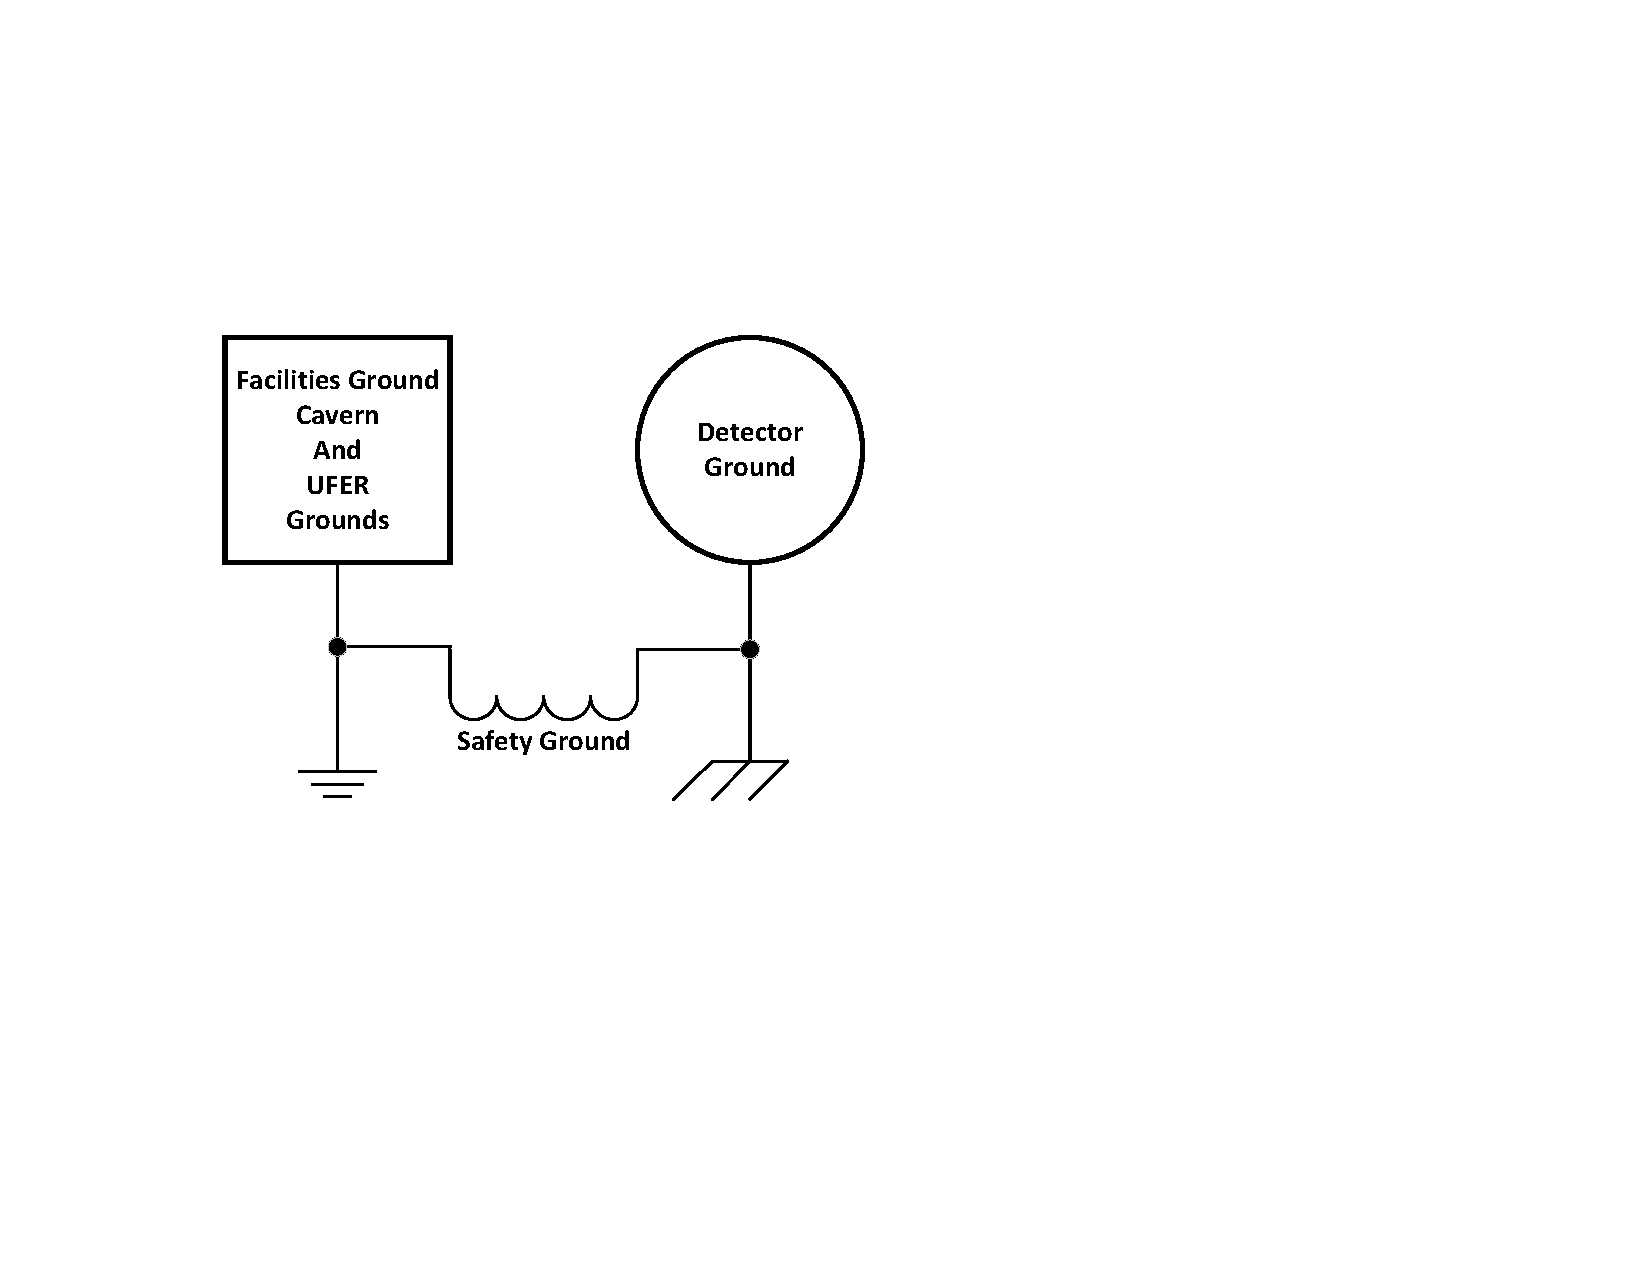
\includegraphics[width=0.5\textwidth]{Simplified_Grounding_Figure.pdf}
\end{dunefigure}


\section{Data Fibers}
\label{sec:fdsp-coord-faci-fibers}


The \dword{dune} experiment has a requirement for a total of sixty-six fiber
optic pairs which run between the surface and the underground.  A
total of 96 fiber pairs, which includes both \dword{dune} and conventional
facility needs, will be supplied through redundant paths with bundles
coming down both the Ross and the Yates shafts.


The experiment has requested a total of fifteen data fiber pairs and
one slow control pair per detector for a total of sixty-four.  Another
two pairs are reserved for GPS.


These fibers are specified to work at 100~Gbps and meet or exceed the
G.652 standard.


\section{Central Utility Cavern Control and DAQ Rooms}
\label{sec:fdsp-coord-cuc-daq}


The Central Underground Cavern (CUC) contains the DAQ and control
rooms for the \dword{dune} experiment.  Both rooms are located in the east
area of the CUC, see Figure~\ref{fig:dune-cuc}.  
\begin{dunefigure}[DAQ and control rooms in CUC]{fig:dune-cuc}
  {Location of underground DAQ and control rooms in the CUC.}
  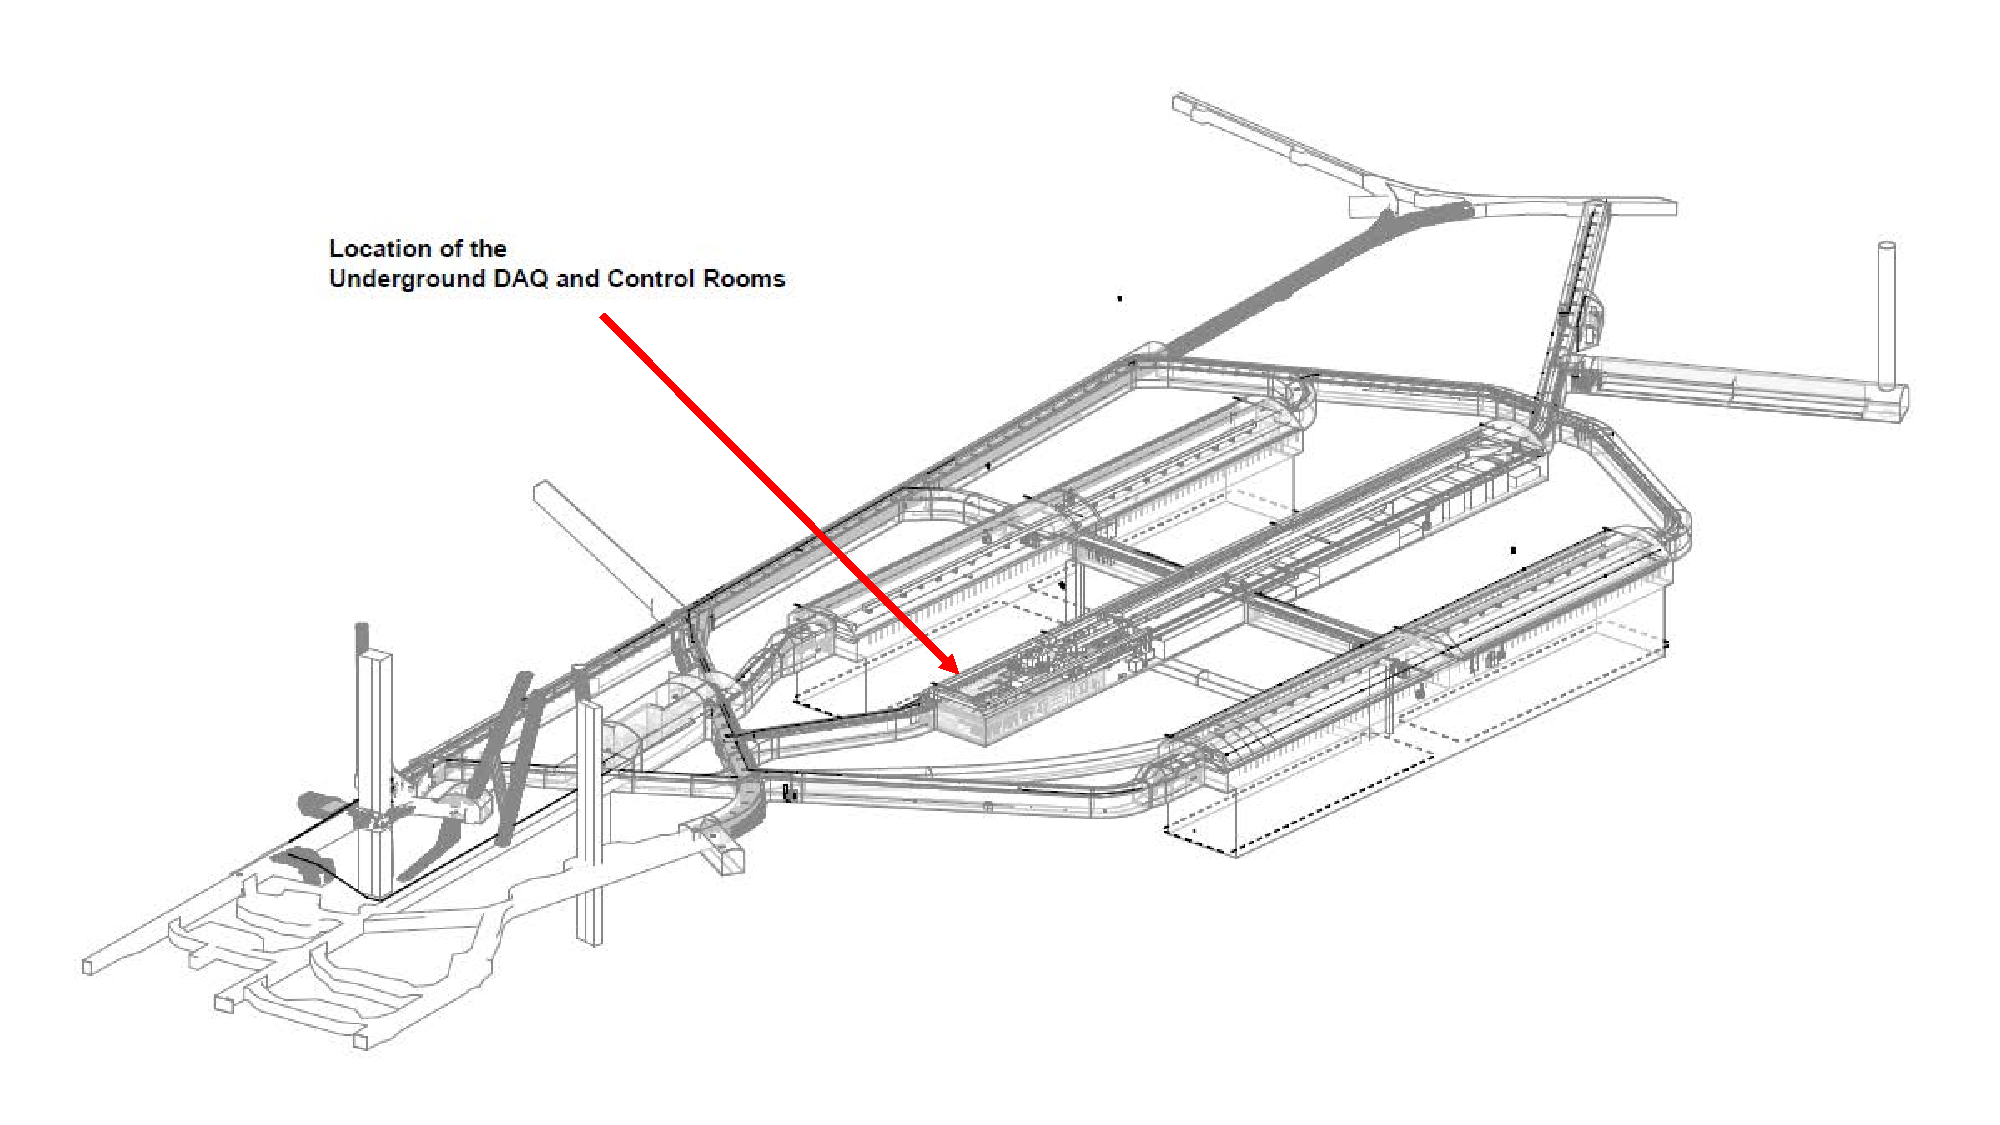
\includegraphics[width=0.85\textwidth]{Location_Underground_DAQ_Control_Rooms.pdf}
\end{dunefigure}
The size and suggested outfitting of the rooms can be seen in
Figure~\ref{fig:dune-daq}.
\begin{dunefigure}[DAQ and control rooms]{fig:dune-daq}
  {Underground DAQ and control rooms layout.}
  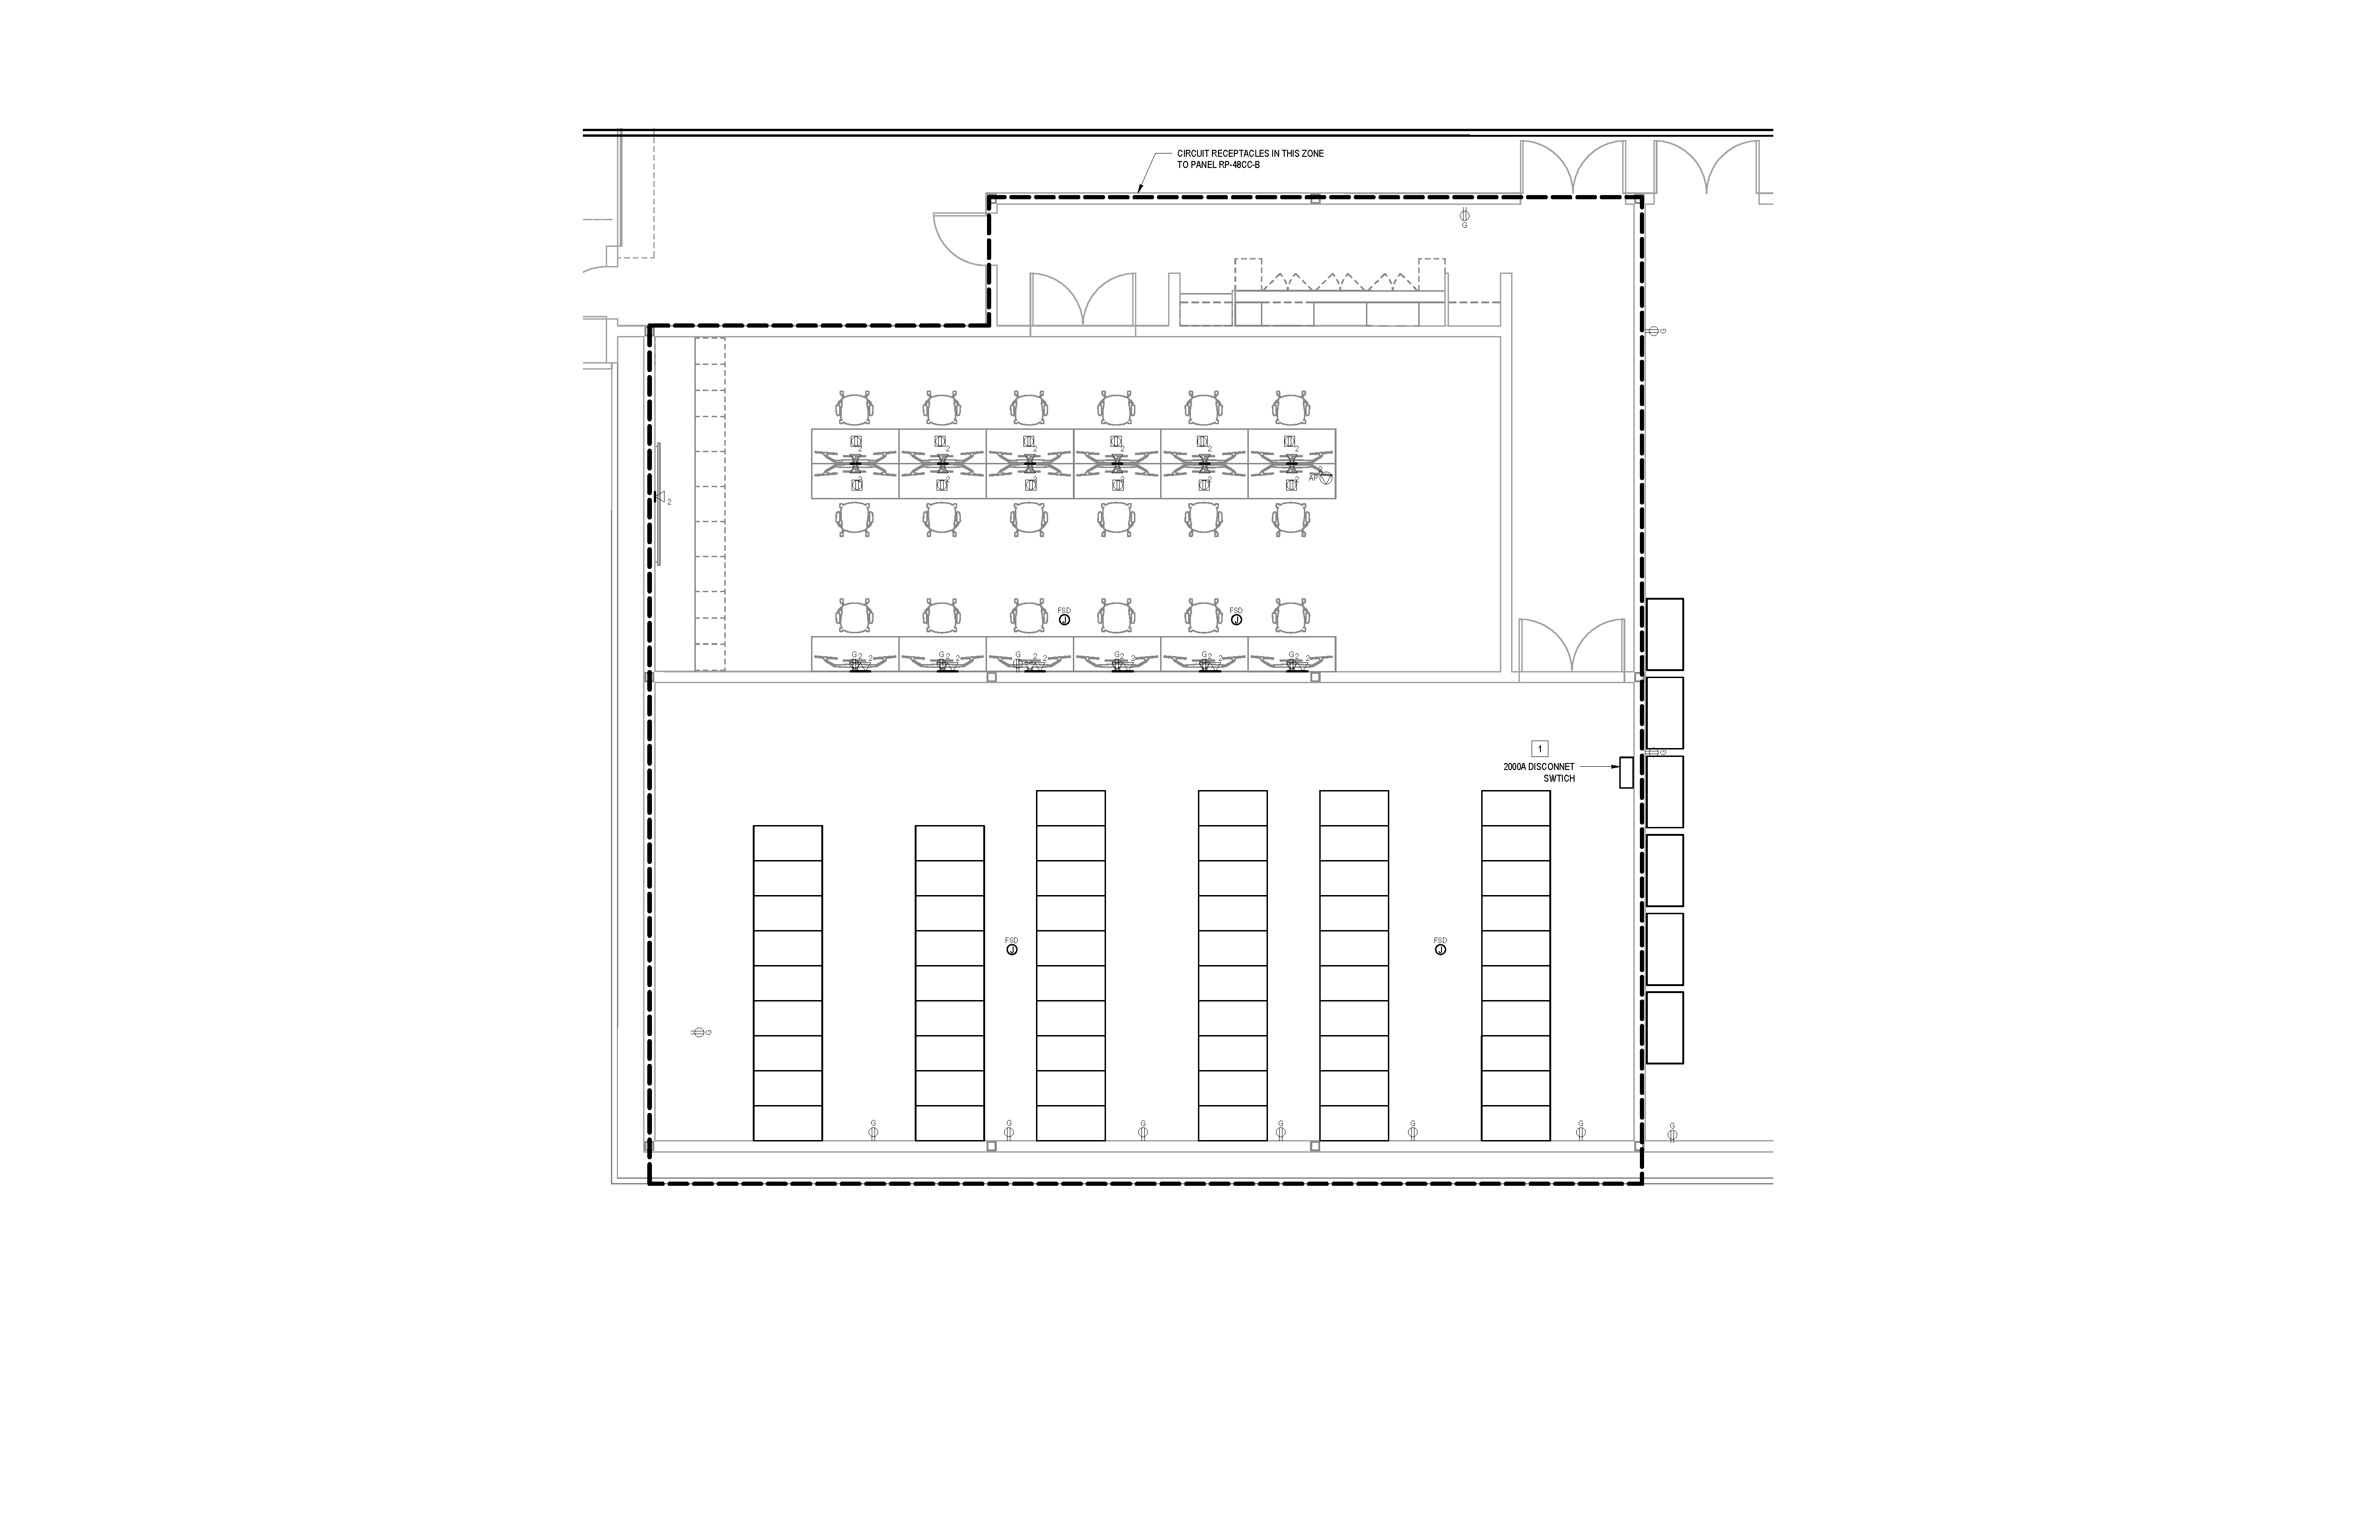
\includegraphics[width=0.5\textwidth]{Preliminary_Layout_DAQ_Control_Rooms.pdf}
\end{dunefigure}


The Control Room is primarily viewed as a meeting or work space where
five to ten people can sit with laptops during system commissioning.
It is not, as its name implies, a Control Room from which the
experiment will be run.  It also provides the required work space for
the cryogenic systems monitoring.  The cryogenic team requires a
footprint of two racks and two work benches for technicians who are
monitoring cryogenic systems.
       
The DAQ room will contain a minimum of 52 racks which will be used for
fiber optic cable distribution, networking, \dword{dune} DAQ, and the
requirements of conventional facilities.  A minimum of 48 racks are
reserved exclusively for DAQ.  Conventional facilities supply the DAQ
room with a tap to cooling water, an 18~inch raised floor, lighting,
HVAC, dry fire protection and 500kVA available power.  Technical
coordination will be responsible for the final outfitting and layout
of the room.  This includes the layout and installation of water
cooled racks, the design and installation of the cooling water piping
to the racks, the AC power distribution to the racks, and installation
of cable trays.


\section{Surface Rooms}
\label{sec:fdsp-coord-surf-rooms}


The \dword{dune} experiment will utilize three surface rooms --- a Surface
Control Room, a DAQ Surface Computer Room and a Facilities Room.


The \dword{dune} Surface Control Room is provided as a host lab
responsibility.  It will be used to commission, monitor and run the
experiment.  This may be a facility which includes shared space with
other experiments taking place at the Sanford Underground Research
Facility.


The DAQ consortia requires a Surface Computer room which will have a
quantity of eight racks and a minimum of 50kVA of power.  Connection
to the optical fibers running through the Ross and Yates shafts as
well as to ESNET will be required.


The Facilities Room is located in the basement of the Ross surface
building.  It will host both the \fnal provided network and
distribution racks for the fibers which run underground. Some details
of this room can be found in Figure~\ref{fig:dune-surf-control}.
\begin{dunefigure}[Surface control rooms]{fig:dune-surf-control}
  {Surface control room.}
  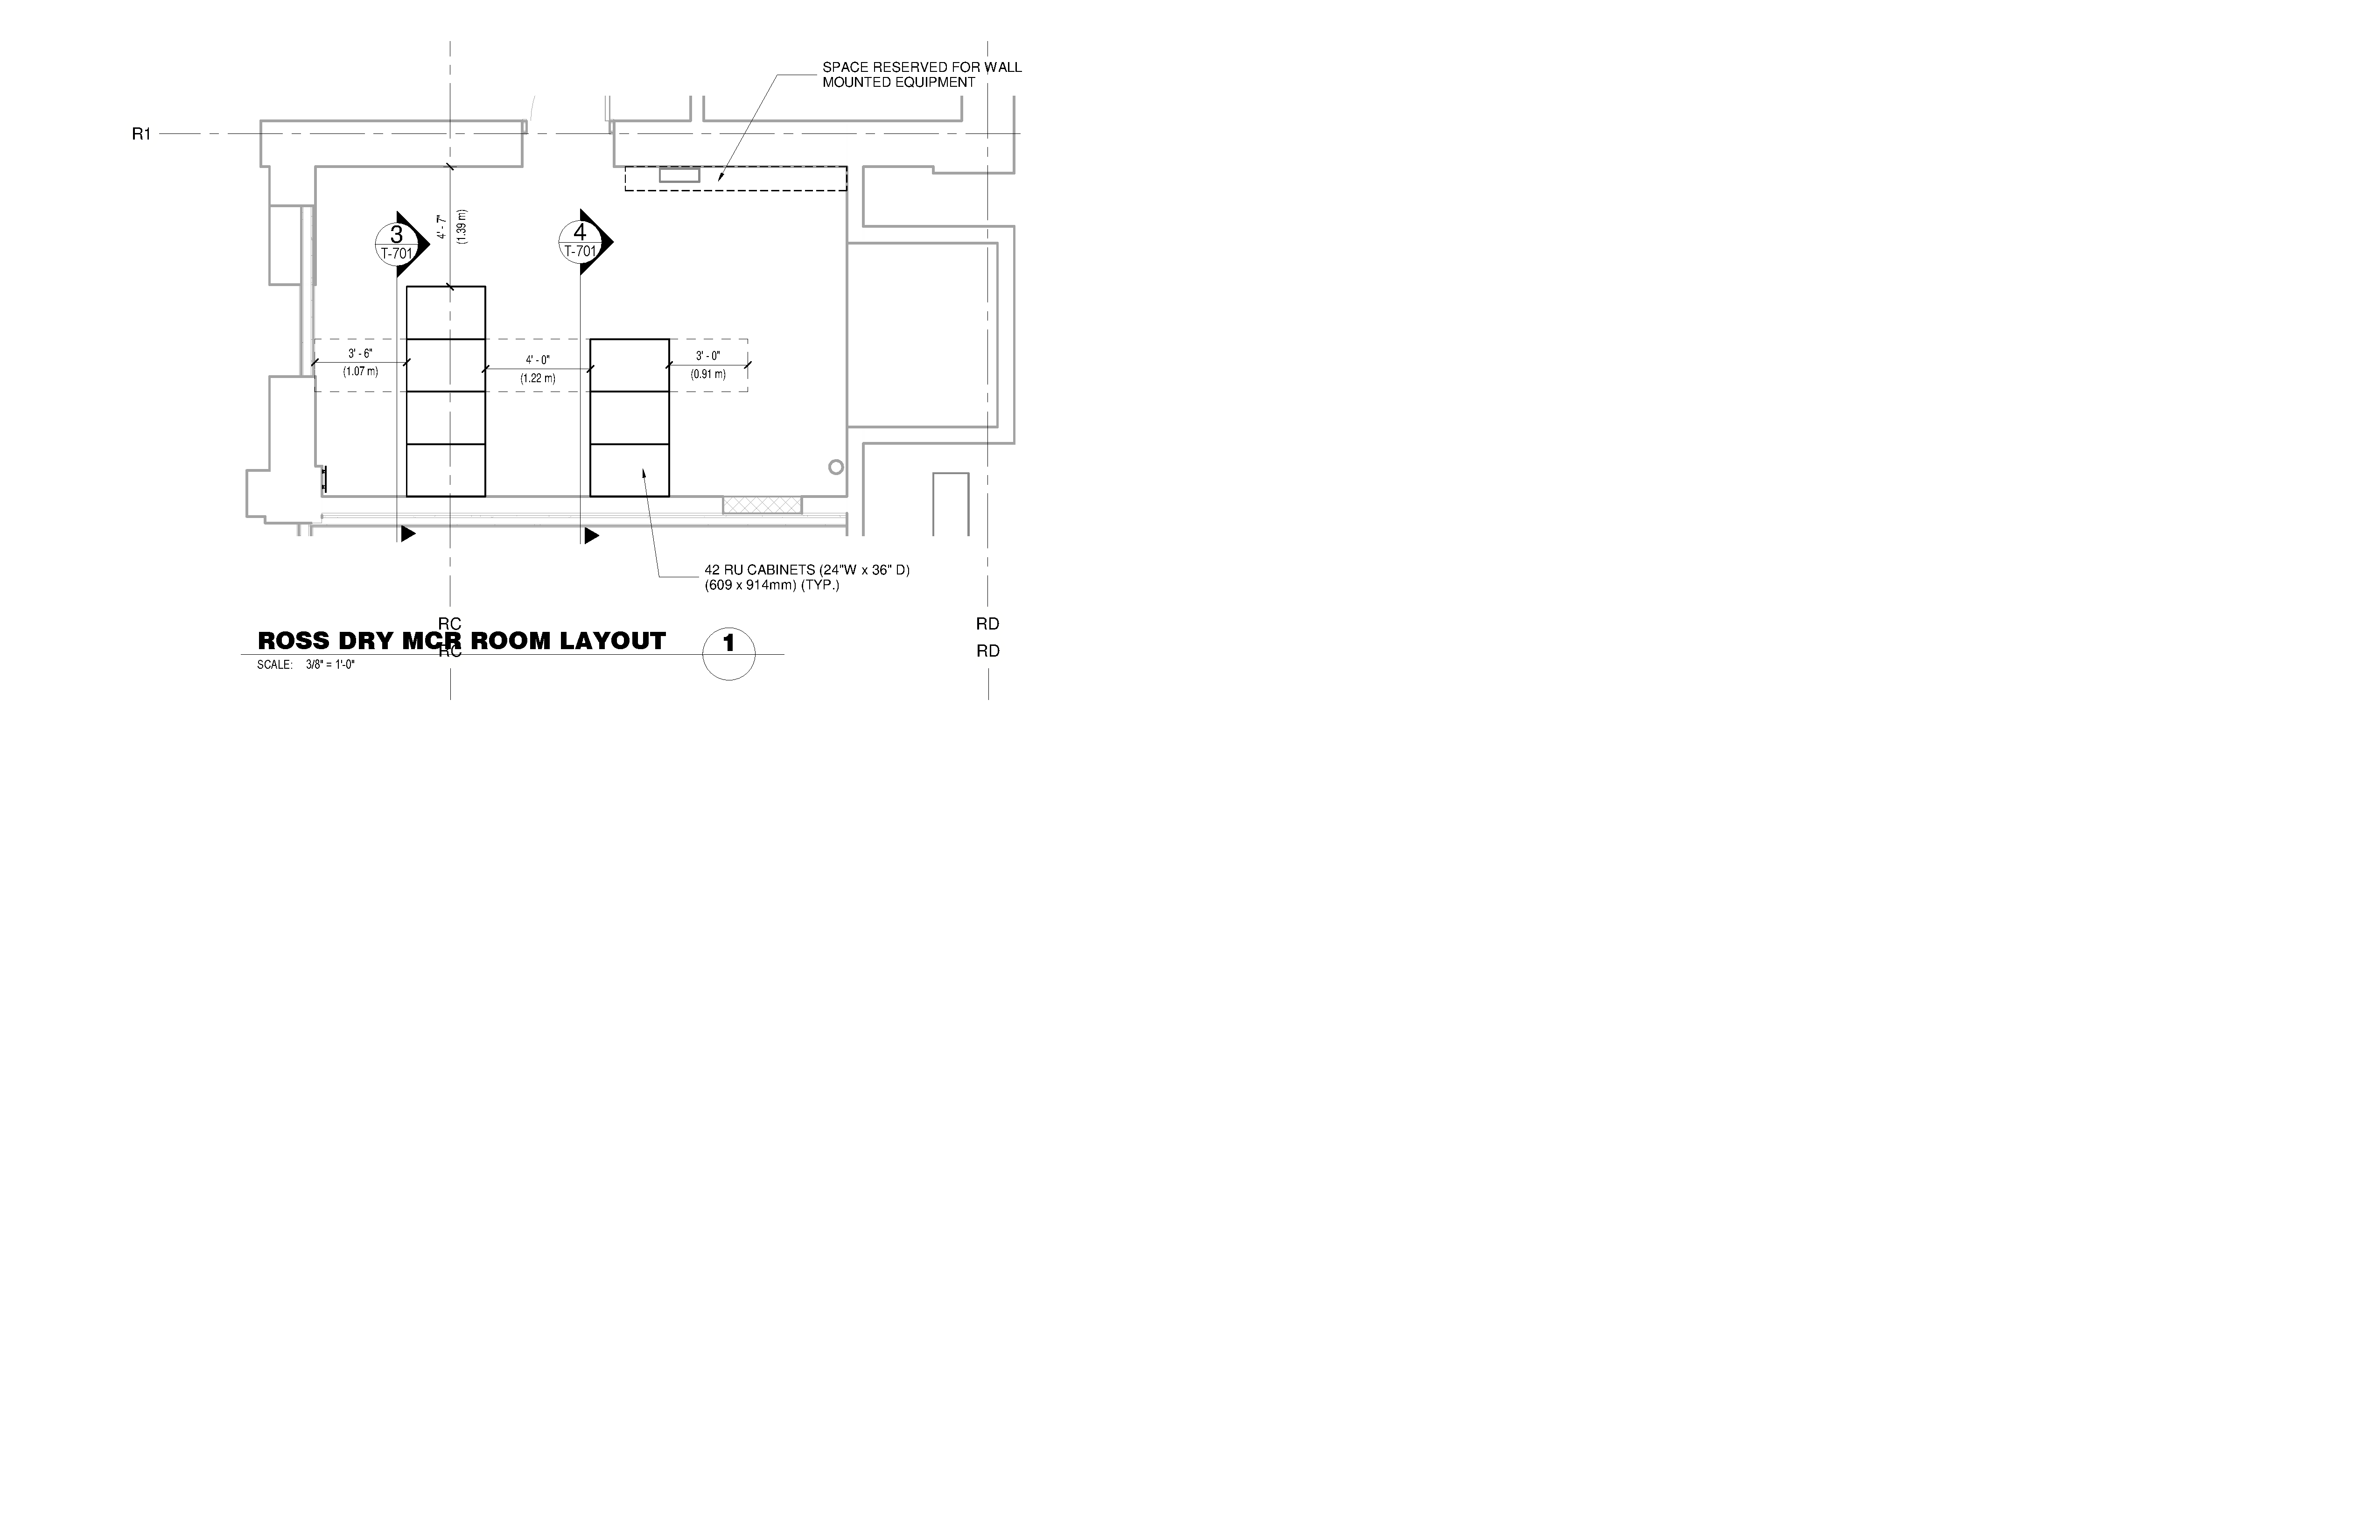
\includegraphics[width=0.85\textwidth]{Surface_Network_Fiber_Optic_Distribution_Room}
\end{dunefigure}


\section{\dword{dune} Detector Safety System}
\label{sec:fdsp-coord-det-safety}


The \dword{dune} Detector Safety System (DDSS) functions to protect
experimental equipment.  The DDSS is required to detect abnormal and
potentially harmful operating conditions.  It must recognize when
conditions are not within the bounds of normal operating parameters
and automatically take pre-defined protective actions.


The DDSS must communicate to the \surf Facility Information
Reporting Utility System (FIRUS) and the \dword{dune} Slow Controls
System which monitors the detector status.  Through communication
links and working together, the three distinct systems provide the
ability to monitor the status of the experiment, protect the equipment
and provide life safety. Figure~\ref{fig:dune-DDSS} indicates how
these systems interact.
\begin{dunefigure}[Detecor Saftey System]{fig:dune-DDSS}
  {Detector Safety System block diagram.}
  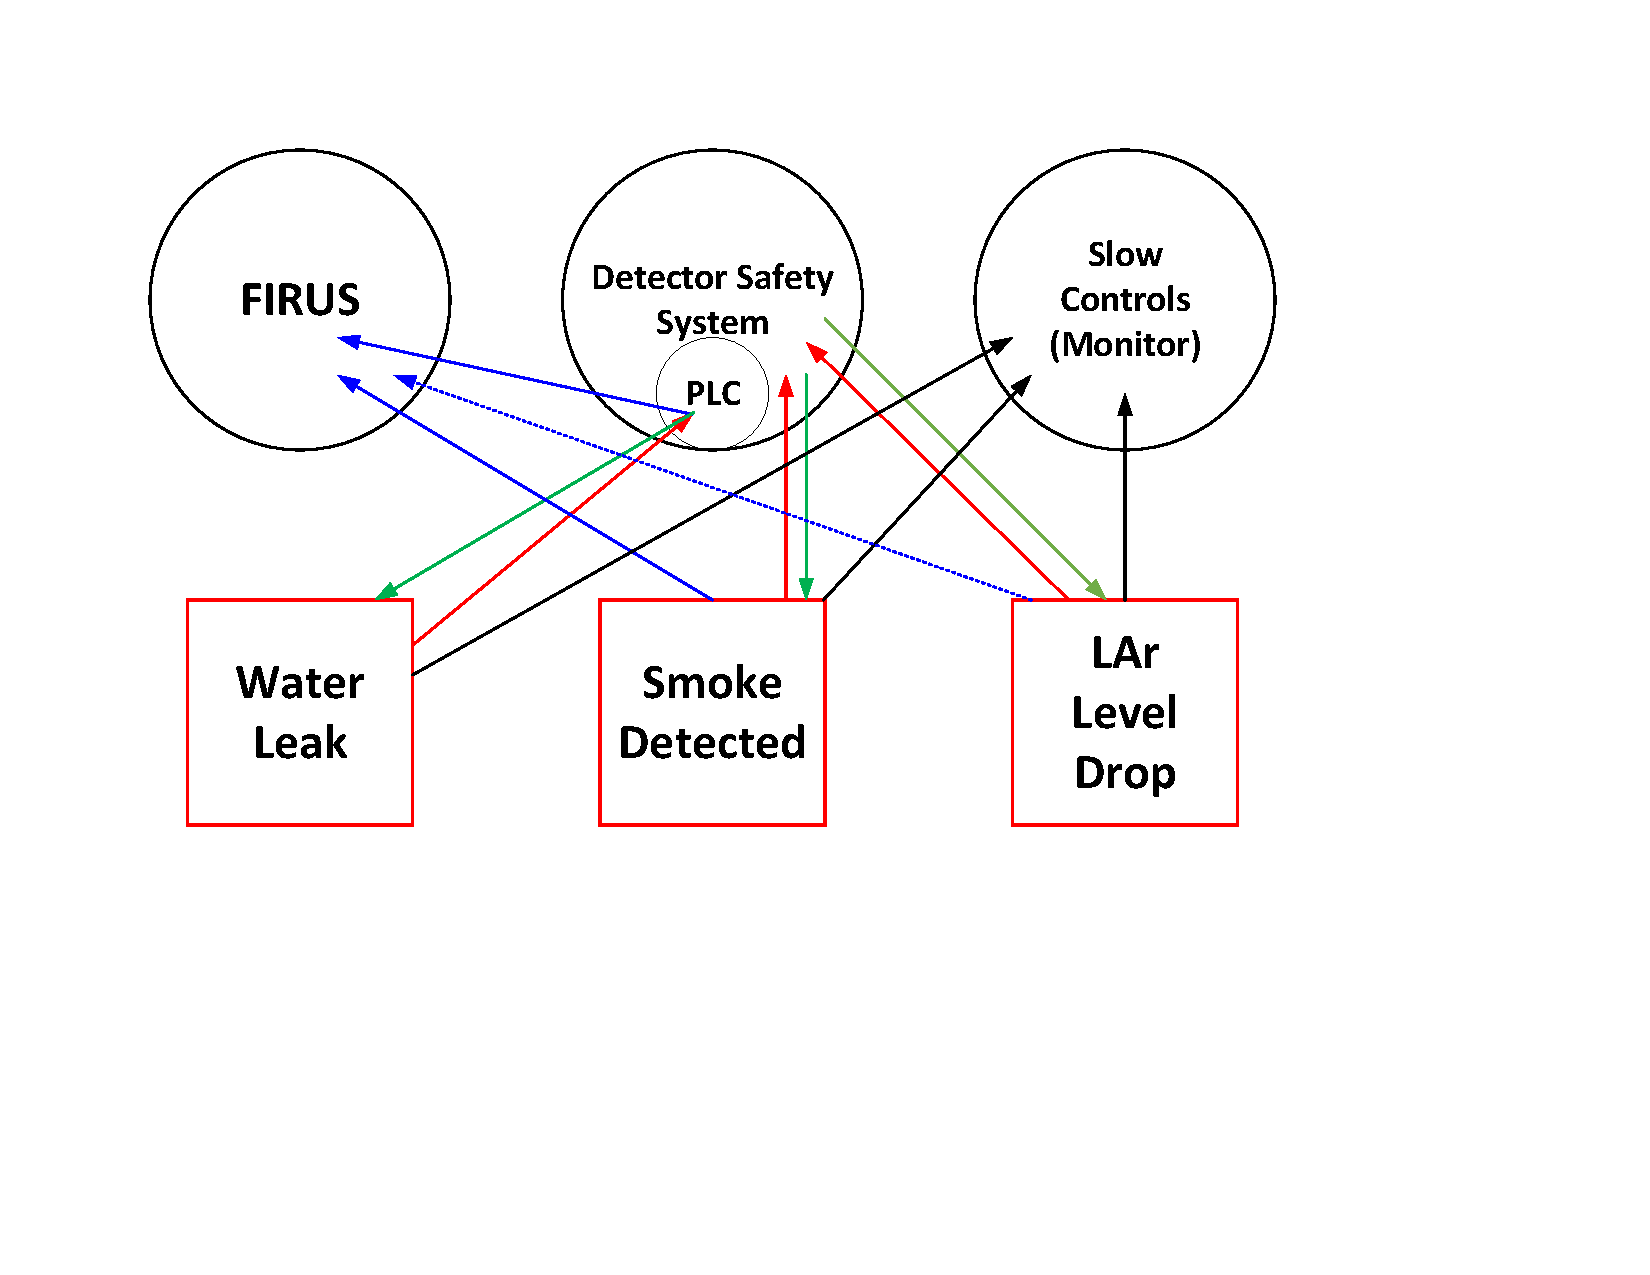
\includegraphics[width=0.85\textwidth]{DSS_Block_Diagram.pdf}
\end{dunefigure}


The DDSS system will be implemented through a combination of
hardware interlocks and the use of a programmable logic controller
(PLC).  Listed below are some of \dword{dune} experimental conditions which
will require the intervention of the DDSS:
\begin{enumerate}
 \item A drop in the LAr level.  This condition requires a hardware
   interlock on the liquid level.  If the level drops below a
   pre-determined level, the drift high voltage must automatically be
   shut off to prevent equipment damage.  Slow Controls would be
   alerted to this condition through normal monitoring.
 \item Smoke, or a temperature/humidity rise above normal operating
   levels is detected inside of a rack or near an instrumented
   feedthrough.  If either of these conditions is detected, local
   power must be switched off. In the case that smoke is detected, a
   dry contact will alert FIRUS.
 \item A water leak detected near energized equipment in the DAQ
   underground data processing room.  Water leak detectors would
   report to the DDSS PLC and a decision will be made to either
   issue an alert or immediately shut power down to the room depending
   on the alert level detected.  This condition would also be reported
   to FIRUS.
\end{enumerate}
  
